\chapter{System design}

The fiber optic doppler optical coherence microscopy system is designed for cost-efficiency, and to meet the measurement requirements of the cochlear research peformed at the Micromechanics Group.

\section{System overview}

\begin{figure}[h!]
\centering
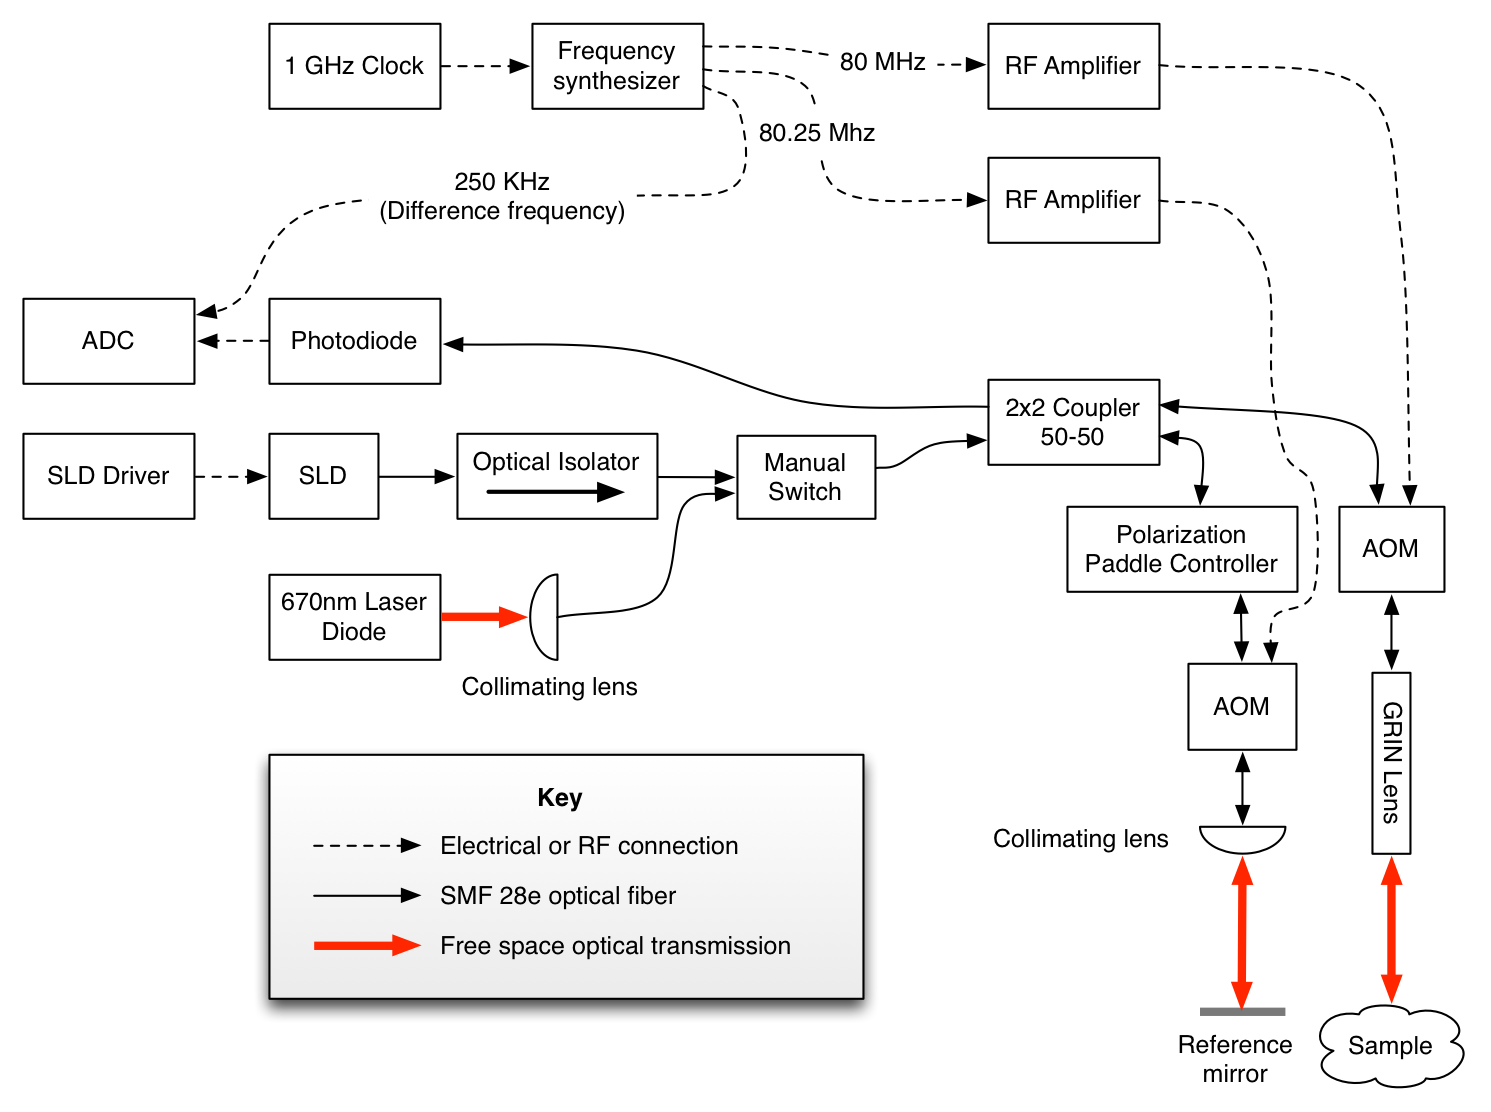
\includegraphics[width=1.1\textwidth]{Images/Background/actual_system_vertical.png}
\caption{Block diagram showing the major components in the fiber optic DOCM system.}
\end{figure}

\subsection{Incoherent light source}

The choice of a light source dictates many aspects of the system performance. The coherence length, as shown in section~\ref{sec:principles_oct}, controls the axial resolution of the imaging. The source is also one of the most expensive components, and therefore plays an important role in determining the overall system cost. The center wavelength of the source relates to what other components may be used in the system, and to the penetration depth achievable.

For this project, we choose an Exalos super-luminescent diode (SLD). Super luminescent diodes provide the spatial coherence of a laser with the temporal incoherence (therefore, short coherence length) of an LED or ``white'' light source.

A center wavelenght of 1310 nm was choosen as this is a common wavelength for communications. It is therefore possible to find many inexpensive fiber coupled components designed to operate in this band.

\begin{table}[h!]
\centering
\begin{tabular}{ >{\bf}r | l}
Part number & Exalos EXS210045-01 \\
Center wavelength & 1310 nm \\
FWHM Bandwidth & 100 nm \\
Coherence length & 7.57 $\mu$m \\
Power & 10 mW \\
Price & \$1800, \$900 driver \\
\end{tabular}
\caption{Specifications for the optical source.}
\end{table} 

\subsection{Acousto-optic modulators}

Two Gooch \& Housego acousto-optic modulators were choosen. Sintec Optronics packages these AOMs in a fiber coupled enclosed package, which avoided the need for alignment with the first degree deflection beam, and provides a convenient, compact device. An 80 MHz drive frequency was choosen for compatibility with existing hardware used in the Micromechanics group. 

\begin{table}[h!]
\centering
\begin{tabular}{ >{\bf}r | l}
Part number & \\
Center wavelength & 1310 nm \\
-3dB Bandwidth & 100 nm \\
Drive frequency & 80 MHz \\
Drive power & 1.5 W \\
Price & 2, at \$1500 each \\
\end{tabular}
\caption{Specifications for the acousto-optic modulator.}
\end{table} 

\subsection{RF Generation and Driving}

The AOMs need to be driven by an 80 Mhz and an 80.25 MHz RF signal in order to produce the beat frequency derived in Section \ref{sec:aom_carrier}.

A 1GHz clock is generated by a Fox Electronics XpressO LVPECL oscillator (part number FXO–PC536R-1000). An output of +13 dbM was measured. This oscillator and the small amount of supporting electrical hardware required was packed in an enclosure and connected to a BNC output.

%% Schematic of 1Ghz oscillator
\begin{figure}[h!]
\centering
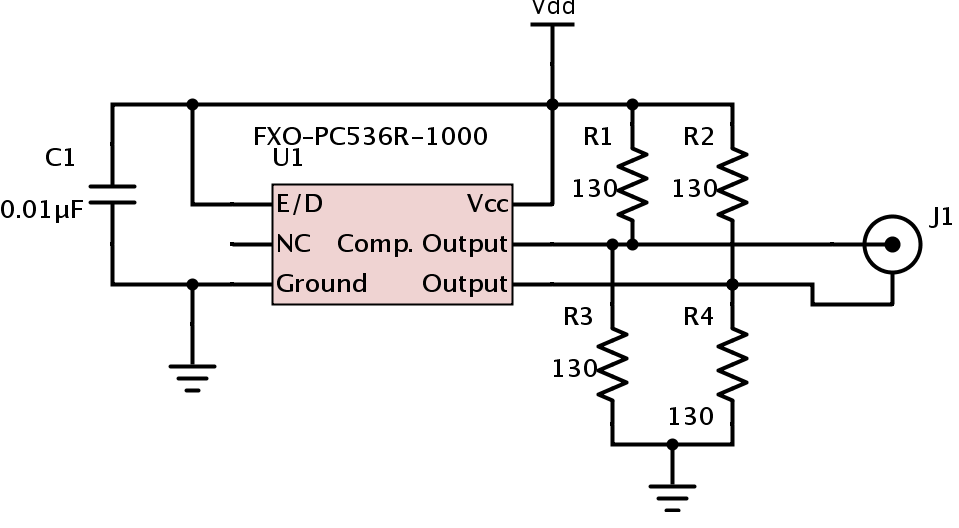
\includegraphics[width=0.75\textwidth]{Images/Schematics/1ghzclock_2.png}
\caption{Schematic of the 1 GHz clock. J1 is the 1 GHz output.}
\end{figure}

A frequency synthesizer, built by Stanley Hong \cite{hong}, uses this 1 GHz clock to synthesize a 80.25 MHz signal and an 80 MHz signal. The difference between these, a 250 Khz signal, is also generated, as it is necessary for signal processing.

Two RF amplifiers, purchased from Mini-Circuits (model ZHL-3A) amplify the RF signals +29.5 dBM to +32 dBm (approximately 1.5 Watts), the maximum drive power of the AOMs.

\subsection{Reference path}

%% Image of reference path setup

The reference path uses a fiber optic collimator purchased from Thorlabs, and focuses it onto an AR-coated retroreflector. A retroreflector was used instead of a mirror for better alignment, as a retroreflector has no sensitivity to the angle offset between the collimated beam and its front surface.

A retroreflector does induce changes in the polarization of the beam, however, the polarization is effectively randomized due to strain and compression in the optical fiber.

\subsection{Sample path objective}

A graded index (or GRIN) lens was used. The GRIN lens is sold by Thorlabs, as a package that can be assembled to focus to a desired distance. This was fixed with Norland Optical Adhesive 68 and cured under UV light.

\begin{figure}[h!]
\centering
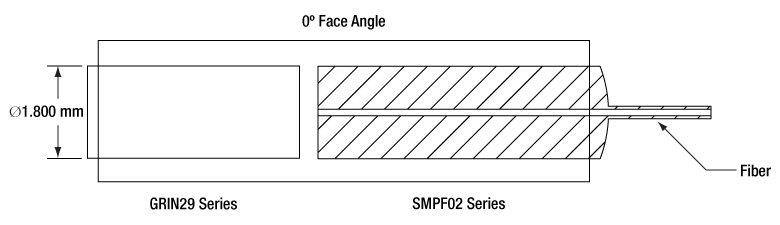
\includegraphics[width=1.0\textwidth]{Images/System/grin.png}
\caption{The GRIN lens assembly. The angled face prevents back-reflection. \em{Image from Thorlabs.}}
\end{figure}

The working distance choosen for the GRIN objective is a tradeoff between the physical distance to the tissue under examination, the working distance $W$, and the conveniences that having this physical distance provides, and the transverse resolution and scattered light amplitude.

%% scattered light amplitude

The solid angle subtended by the GRIN lens is equal to

\begin{equation}
\Omega = 2 \pi (1 - \cos{\theta})
\end{equation}

where $\theta = \arctan{\frac{r_{grin}}{W}}$.

\begin{equation}
\Omega = 2 \pi \left(1 - \sqrt{\frac{W^2}{W^2 + r_{grin}^2}} \right)
\end{equation}

Assuming an isotropic scatterer, the fraction of optical power that will be recollected by the GRIN lens is equal to $ \left( \frac{\Omega}{4 \pi} \right)^2 $. As the GRIN lens used in this thesis has a radius of 0.9mm, this fraction may be written numerically as follows.

\begin{equation}
\frac{1}{4} \left( 1 - \sqrt{\frac{W^2}{W^2 + 0.81}} \right) ^ 2
\end{equation}

A plot of this value for working distances between 0 and 5 mm is shown below.

\begin{figure}[h!]
\centering
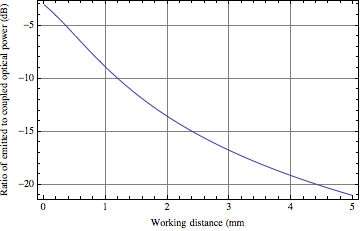
\includegraphics[width=1.0\textwidth]{Images/System/grin_scattering.png}
\caption{Captured light ratio as a function of working distance, in mm.}
\end{figure}

As previously discussed in Equation \ref{eq:tres}, the axial resolution is given by:

\begin{equation} \label{eq:tres2}
\delta_x = 0.61 \frac{\lambda}{NA} \approx 1.22 \frac{\lambda W}{1.8 \mathrm{mm}} \approx W \cdot 0.888 \cdot 10^{-3} \;\;
\end{equation}

A working distance of 2 mm was choosen, resulting in a transverse resolution of 1.78 microns, and a reflection loss of -27.1 dB (again, assuming an isotropic scaterrer).

\section{Sample alignment apparatus}

%% solidworks images and mechanical design discussion

\begin{figure}[h!]
\centering
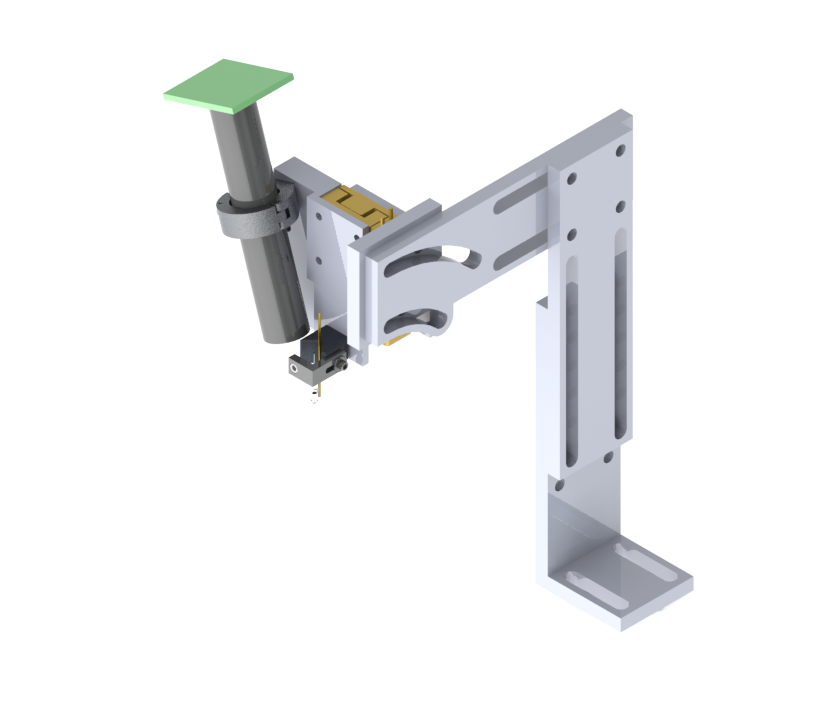
\includegraphics[width=1.0\textwidth]{Images/Alignment/new_d_2.png}
\caption{A SolidWorks model of the mechanical alignment apparatus.}
\end{figure}

The sample alignment apparatus is a mechanical device designed to satisfy several goals:

\begin{itemize}
	\item Securely hold the GRIN objective lens
	\item Move the GRIN objective along the direction of the optical axis with a precise motorized stage
	\item Allow the GRIN objective lens to be rotated a certain angle around its focal point
	\item Allow coarse adjustments for height and cantilever distance
	\item Provide a visible alignment aid beam
	\item Hold a small digital microscope for visual inspection of alignment
\end{itemize}

\subsection{Mechanical device for adjusting angle}

To control the angle, the z-stage is mounted on a horizontal aluminum cantilever, with two circularly concentric slots cut out. By screwing the stage mounting block into the slots, the angle can be adjusted around a fixed point. When the system is configured such that it is focused on this point, the operator is able to change the angle of axial movement without changing the current focal point, a helpful feature for alignment.

\begin{figure}[h!]
\centering
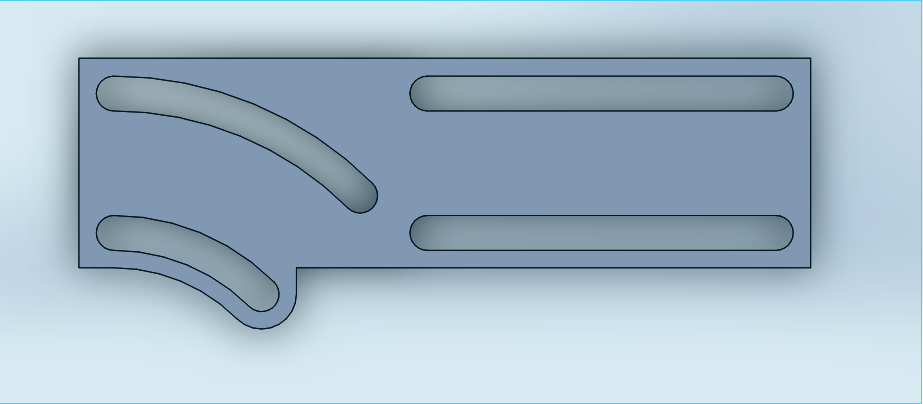
\includegraphics[width=1.0\textwidth]{Images/Alignment/horizontal_part.png}
\caption{The horizontal cantilever piece, with two slots allowing for angular adjustment.}
\end{figure}

The cantilever part was designed in SolidWorks and then CNC milled in the Edgerton Center Student Shop.

\subsection{Piezo motor stage for axial movement}

\begin{figure}[h!]
\centering
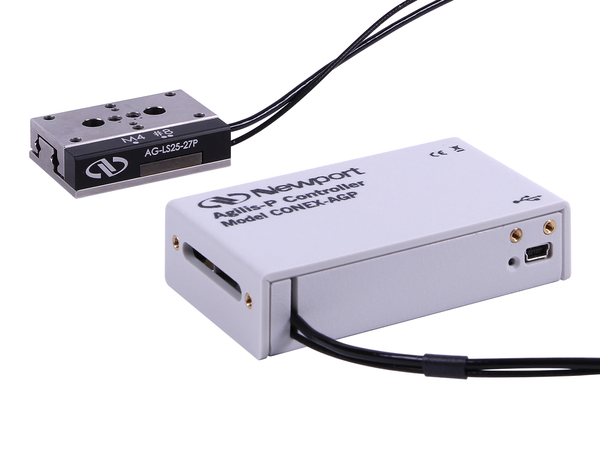
\includegraphics[width=0.48\textwidth]{Images/System/z-stage.jpg}
\caption{The piezo motor stage with controller.}
\end{figure}

\begin{table}[h!]
\centering
\begin{tabular}{ >{\bf}r | l}
Part number & CONEX-AG-LS25-27P\\
Travel range & 27mm  \\
Repeatability & 200 nm \\
Speed & 0.4mm / sec \\
Minimum incremental motion & 200nm \\
Price & \$1725 \\
\end{tabular}
\caption{Specifications for the axial piezo motor stage.}
\end{table}

To control $z$-axis scanning, a piezo-electric motorized stage was used. This stage uses an ``inchworm'' like drive method to control motion, and uses motion encoders with closed loop feedback to provide repeatable movements of up to 200 nm.

Unfortunately, this stage also had some drawbacks for an OCT application. Though the closed loop feedback allows for the stage to move precisely to any location, it's speed is not consistent during the motion. As a result, it is necessary to re-interpolate the data collected based on the actual position of the stage as it scans. This is discussed further in the signal processing section, Section \ref{sec:sig_proc}.

To capture information about the realtime position of the stage two approaches were used. The first involved repeatedly querieing the CONEX stage driver over tty serial. While this was straightforward to accomplish and within the bounds of normal operation of the stage, it did not provide high enough resolution (in time) of the stages' position.

The second approach involved adding analog output from the stage encoder that could be captured by the analog-to-digital converter simultaneously with the interferometry signal. This involved ``hacking'' % should I use this word?
the controller.

\begin{figure}[h!]
\centering
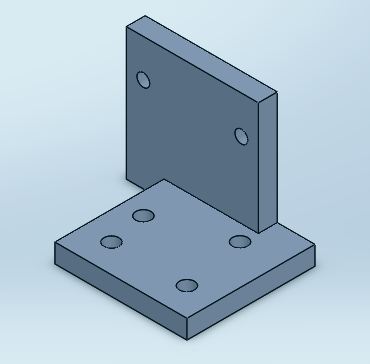
\includegraphics[width=0.48\textwidth]{Images/Alignment/angle_bracket2.png}
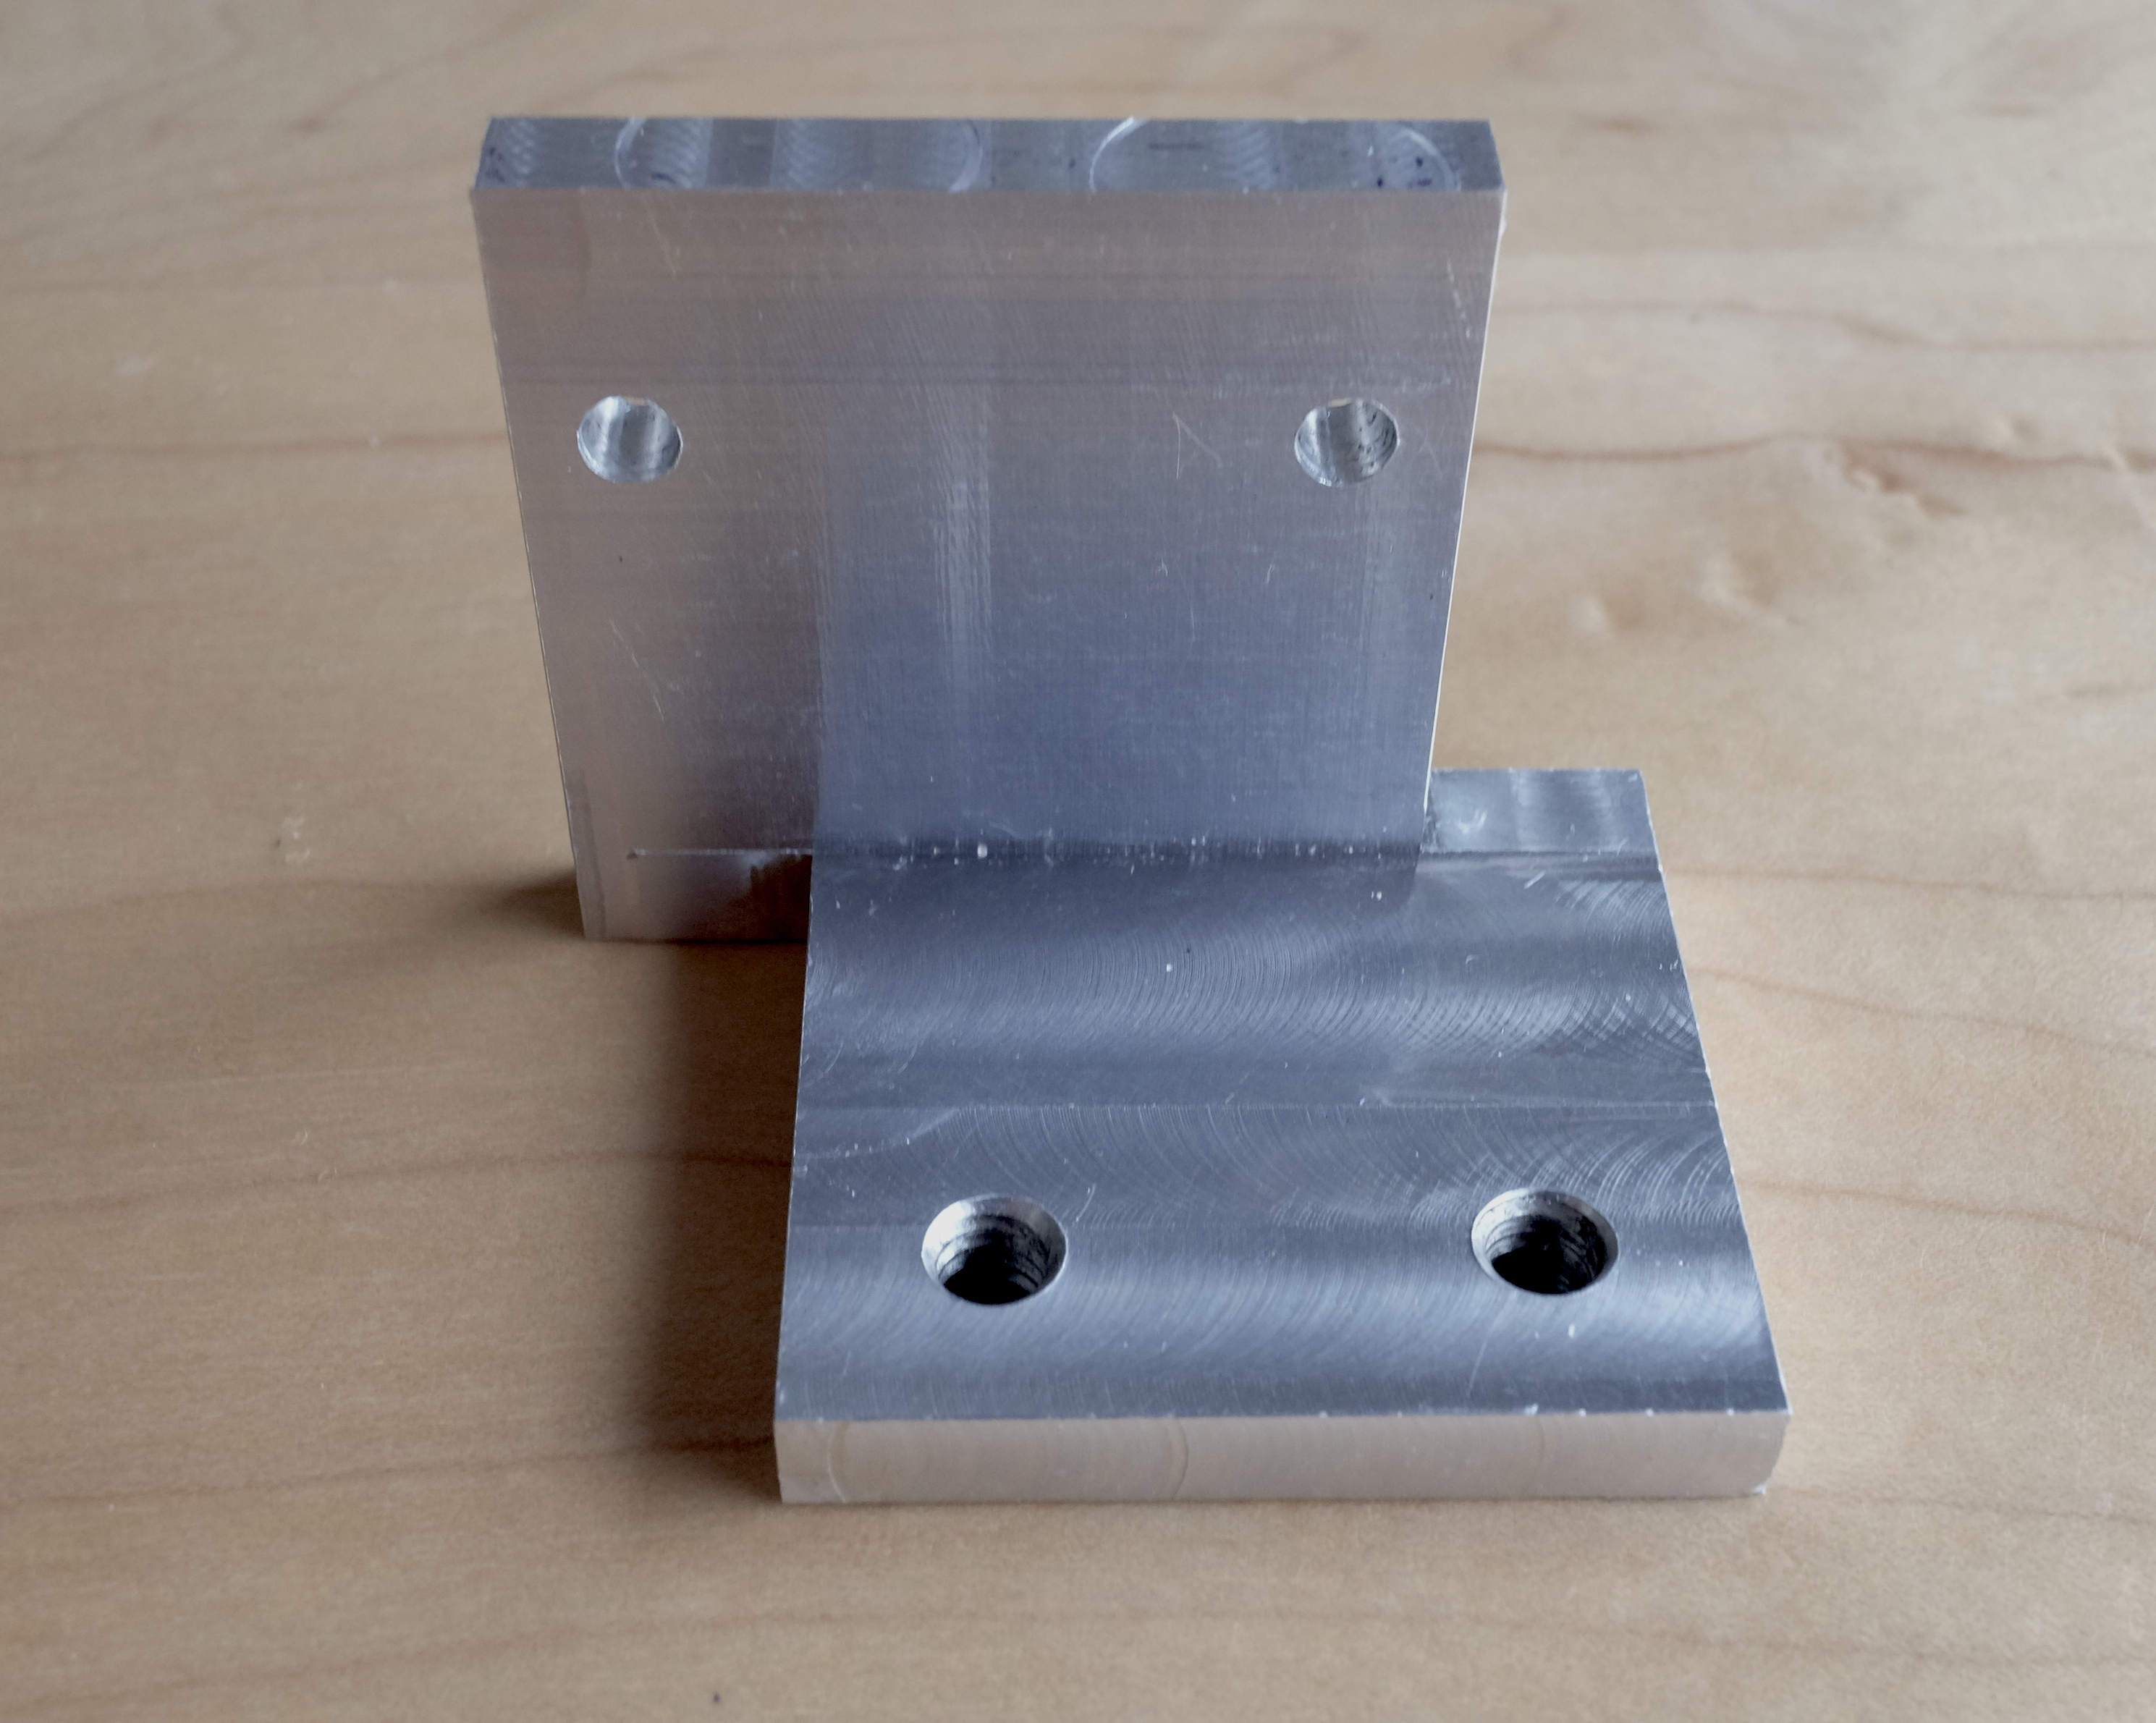
\includegraphics[width=0.48\textwidth]{Images/Alignment/angle_bracket.jpg}
\caption{This angled bracket mounts the piezo-motor stage to the horizontal cantilever shown above. The image on the right shows the bracket prior to the addition of stabilization bolts.}
\end{figure}

\subsection{Mounting the fiber and GRIN lens}

\begin{figure}[h!]
\centering
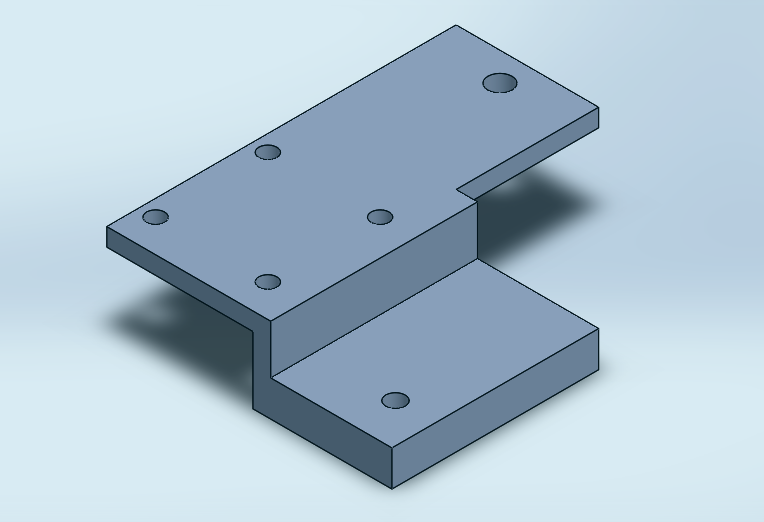
\includegraphics[width=0.75\textwidth]{Images/Alignment/mounting_plate.png}
\caption{This mounting bracket fastened to the z-stage and allowed the installation of a Thorlabs V-clamp.}
\end{figure}

To hold the fiber and its objective GRIN lens, a Thorlabs V-clamp was used. A custom part was designed in SolidWorks to connect to the piezo stage, allow the V-clamp to be mounted, and also to allow the digital microscope to be installed such that it could image the focal point of the GRIN lens. This part was designed in SolidWorks, and then milled by hand in the Edgerton Center Student Shop.

\subsection{Digital microscope for visual alignment}

%% Image of final microscope

In order to aid the alignment process, an optical microscope, with a digital CCD view finder, was created to observe the region imaged by the OCT process.

The design required a relatively large working distance (and correspondingly low numerical aperture), to allow the microscope to have an angle as close to the optical axis of the OCT objective lens as possible.

A CCD sensor from a Microsoft Xbox Live Vision web camera was used, due to its compact size, low cost, and use of standard, MATLAB compatible protocols for transferring images. As the CCD has a quite small size, approximately 3x5mm (actual dimension specifications are not available), a low magnification was sufficient.

A MATLAB program was ued to optimize the working distance, while keeping the overall optical length within reasonable limits, and while working with a set of easily obtainable lenses, using a simple paraxial lens approximation. From this MATLAB program, a ZEMAX simulation model was constructed, using accurate models of the actual lenses from which the microscope would be constructed.

The microscope is composed of three lenses in two groups -- a 15mm spherical doublet (Edmund 45209) and a 20mm spherical singlet (Thorlabs LA1074). The lenses are mounted in $1/2$ inch $\diameter$ lens tubes.

\begin{figure}[h!]
\centering
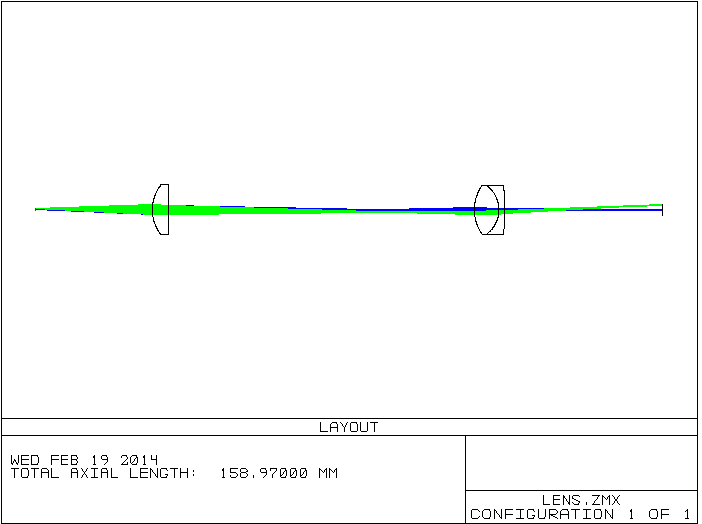
\includegraphics[width=0.8\textwidth]{Images/Microscope/microscope_layout.png}
\caption{A raytrace diagram of the microscope layout, simulated in ZEMAX.}
\end{figure}

\begin{figure}[h!]
\centering
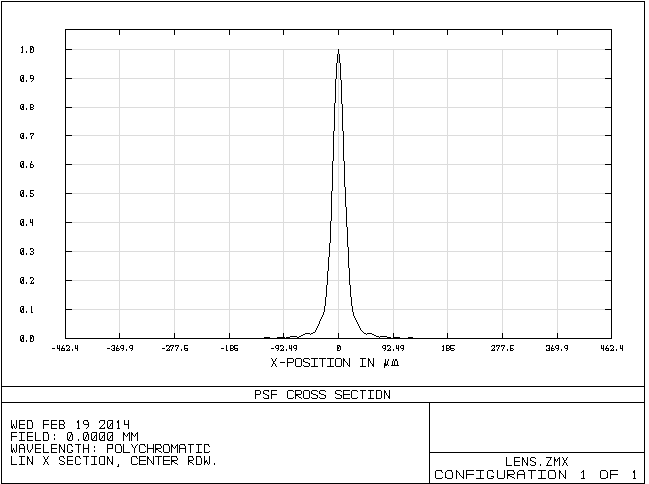
\includegraphics[width=0.8\textwidth]{Images/Microscope/microscope_psf.png}
\caption{The point spread function of the microscope, as simulated in ZEMAX. Note the actual performance was slightly better than in the simulation.}
\end{figure}

The performance was tested using a 1961 USAF Resolution Test Target, which showed that the microscope could resolve features down to 7.8 microns wide, and had a field of view of 1.16 mm $\times$ 0.87 mm, for a magnification of approximately 4$\times$.

\begin{figure}[h!]

\centering
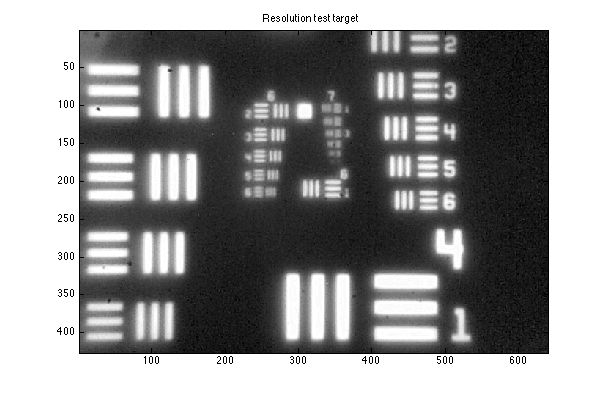
\includegraphics[width=1.0\textwidth]{Images/Microscope/target.png}
\caption{An image of a 1961 USAF Resolution Test Target, taken using the digital microscope. \label{fig:usaf}}
\end{figure}

While the performance of this microscope would not be considered ``great'' for any serious imaging applications (in particular, the contrast is quite poor, as evidenced by the ``haze'' around the bright regions in Figure \ref{fig:usaf}), it is sufficient for performing the basic alignment of the OCT appartus, and therefore is sufficient for the design requirements. Due to the nature of the microscope's application, the sample is not illuminated by transillumination, but instead by simply viewing the light scattered off of the sample from a bright LED source, mounted near the end of the microscope. Again, while this is not optimal for imaging applications, it meets the design requirements as an alignment microscope.

\subsection{Visible laser for assisting visual alignment}

%% Image of laser

The spectral responsivity of a silicon photo-sensor, like that used in the digital microscope CCD, falls sharply above 1000nm. As the optical source in this system is centered at 1310nm, it is difficult to view the spot produced by the focused infrared light. For this reason, a second optical source can be coupled into the GRIN lens.

For this purpose, an inexpensive 650nm laser diode is used. The output of the diode is collimated and coupled into an SMF-28e+ optical fiber, which can be attached through a FC-APC connector directly to the GRIN lens. This produces a highly visible laser spot that is helpful for aligning the start of an OCT scan.

%% Image of laser spot

\section{X-Y stage for sample movement}

To move in the transverse plane, the sample is placed on a stepper motor driven two axis stage. For this purpose, a Prior H101B stage was used. While this stage is designed for use on a conventional upright microscope, some custom mounting hardware was designed and manufactured to allow it to stand freely. The stage is driven by a Prior H128 controller, which accepts commands over a serial port.

\begin{figure}[h!]
\centering
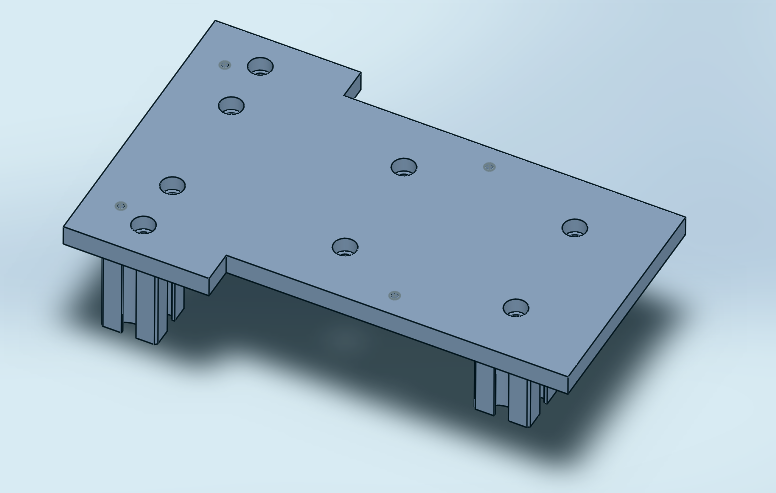
\includegraphics[width=0.75\textwidth]{Images/Alignment/x-y-mount.png}
\caption{The mounting plate designed to allow the Prior H101B microscope stage to stand freely. This was fabricated by laser cutting acrylic.}
\end{figure}

\begin{table}[h!]
\centering
\begin{tabular}{ >{\bf}r | l}
Part number & \\
Center wavelength & 1310 nm \\
-3dB Bandwidth & 100 nm \\
Drive frequency & 80 MHz \\
Drive power & 1.5 W \\
Price & 2, at \$1500 each \\
\end{tabular}
\caption{Specifications for the X-Y stage.}
\end{table} 


\section{Light detection and analog-to-digital conversion}

The light is detected by a Newport New Focus 2117-FC photodiode with an integrated trans-conductance amplifier. This photodiode has a sensitivity range of 900-1700nm, and a transimpedance gain of up to $18.4 \times 10^6 \;\; \mathrm{V}/\mathrm{A}$.

\begin{figure}[h!]

\centering
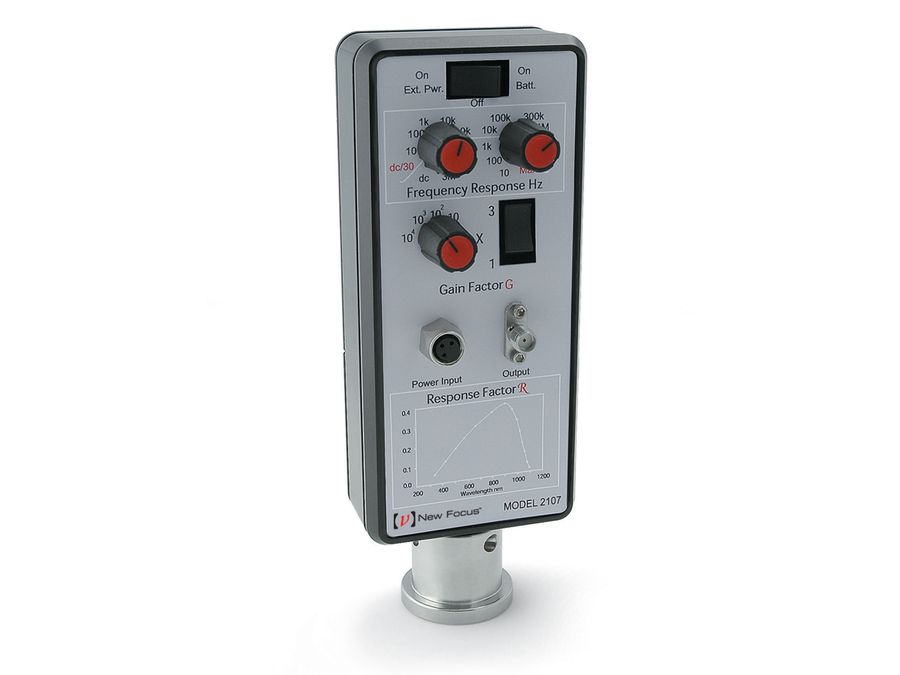
\includegraphics[width=0.6\textwidth]{Images/System/pd.jpg}
\caption{The Newport New Focus 2117-FC photodetector.}
\end{figure}

\begin{table}[h!]
\centering
\begin{tabular}{ >{\bf}r | l}
Part number & \\
Center wavelength & 1310 nm \\
-3dB Bandwidth & 100 nm \\
Drive frequency & 80 MHz \\
Drive power & 1.5 W \\
Price & 2, at \$1500 each \\
\end{tabular}
\caption{Specifications for the photo detector.}
\end{table} 

\section{Signal processing}
\label{sec:sig_proc}

There are two distinct tasks that the OCT system will be required to and capable of performing. One is image generation -- creating a static 2D or 3D image of the sample. The other is motion analysis, capturing information about the movement of one specific area of a sample. The primary difference in these two tasks is that motion analysis requires a period of data to be sampled from one point, while image generation uses a continually scanning axis.

%% Mostly MATLAB and source code here. Theory behind the processing is introduced in Chapter 1

\subsection{Image generation}

An overview of the signal processing steps necessary on acquired data for a single z-axis sweep is shown in Figure \ref{fig:imagegen}.

\begin{figure}[h!]
  \centering
\begin{tikzpicture}[node distance = 2cm, auto]
    % Place nodes
    \node [block] (hilb) {Hilbert transform envelope extraction};
    \node [block, left of=hilb, node distance=3.5cm] (dbpf) {Digital band pass filter};
    \node [cloud, left of=dbpf, node distance=4cm] (pd) {Photodiode signal};
    \node [cloud, below of=pd, node distance=3cm] (enc) {Quadrature encoder signal};
    \node [block, below of=hilb, node distance=3cm] (reint) {Position reinterpolation};
    \node [block, below of=reint, node distance=3cm] (ds) {Downsampling};
    % Draw edges
    \path [line, thick] (pd) -> (dbpf);
    \path [line, thick] (dbpf) -> (hilb);
    \path [line, thick] (enc) -> (reint);
    \path [line, thick] (reint) -> (ds);
    \path [line, thick] (hilb) -> (reint);
\end{tikzpicture}
\caption{A block diagram overview of the steps necessary for image generation. \label{fig:imagegen}}
\end{figure}

\subsection{Motion analysis}

%%%%%%%%%%%%%%%%%%%%%%%%%%%%%%%%%%%%
%%%%%% SECTION 2 PERFORMANCE %%%%%%%
%%%%%%%%%%%%%%%%%%%%%%%%%%%%%%%%%%%%
\section{Theoretical performance predictions}
\label{sec:theory_res}

\subsection{Axial resolution}
\label{sec:axial_res}

Axial resolution is limited by the coherence length of the optical source, as derived in Equation \ref{eq:ares} in Chapter 1. This result is repeated below:

\begin{equation} \label{eq:ares2}
\delta_z = l_c = \frac{2 \ln{2}}{\pi} \frac{\lambda_0^2}{\Delta \lambda}
\end{equation}

The specifications for the optical source used in this project were not precisely equivalent to the measured performance of the actual source. The actual -3dB bandiwdth was 86.3 nm, whereas the specified was 100 nm. Additionally, the actual power output was 7.00 mW, whereas the specified was 10 mW. The results of optical spectrum measurement for this source is shown below.

% Optical spectrum analyzer graph
\begin{figure}[h!]
\centering
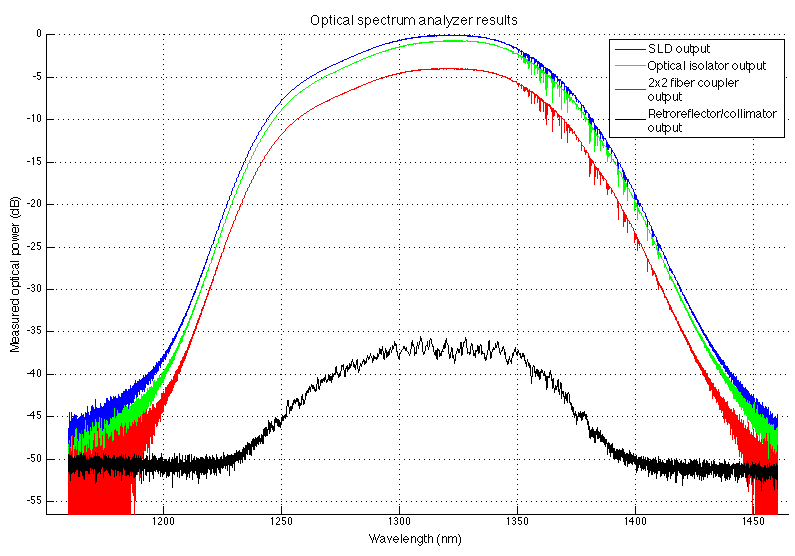
\includegraphics[width=1.0\textwidth]{Images/System/osa.png}
\caption{Optical spectrum analyzer results for the outputs of four critical parts in the OCT system. Due to a different experimental setup, the power levels measured in retro-reflector collimation are not representative of the actual system, and are clearly heavily affected by the noise floor of the optical spectrum analyzer. \label{fig:osa}}
\end{figure}

The slightly smaller bandwidth results in a slightly inferior axial resolution prediction of 8.77 microns. The designed axial resolution (based on data from the Exalos datasheet) was 7.57 microns.

This resolution is not adversally impacted by any other optical components in the system. The results of optical spectrum measurement at the output of several key components in the OCT system are shown in Figure \ref{fig:osa}.

% More OSA graphs?

\subsection{Transverse resolution}
\label{sec:transverse_res}

The maximum achievable resolution in the transverse direction is determined by the diffraction limit:

\begin{equation} \label{eq:tres2}
d = n\frac{\lambda D}{2f}
\end{equation}

where $D$ is the diameter of the entrance aperture, and $f$ is the working distance of the lens (distance to focal point). For the system described above, this evaluates to a diffraction limit of 590 nanometers.

Using ZEMAX Optical Design Software, and files provided from Thorlabs, the manufacturer of the GRIN lens, a more accurate simulation was created of the objective lens performance. Here, it was found to be diffraction limited when an object was on the optical axis (as is the case when emerging from an optical fiber).

\begin{figure}[h!]
\centering
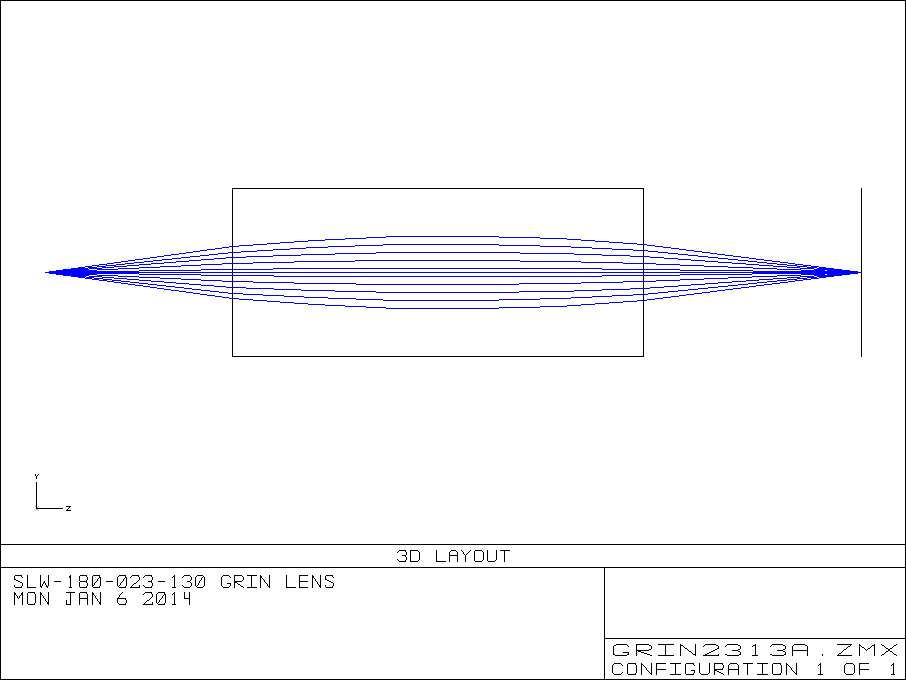
\includegraphics[width=0.75\textwidth]{Images/Zemax/GRO-raytrace.png}
\caption{A ZEMAX raytrace showing the path of light through the GRIN lens. Light emerges from the SMF-28e fiber (NA = 0.14) on the left, and is focused to a point on the right.}
\end{figure}

\begin{figure}[h!]
\centering
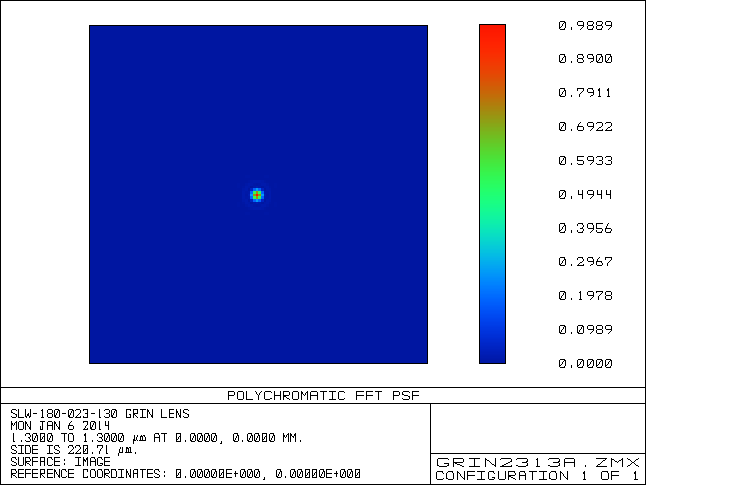
\includegraphics[width=0.75\textwidth]{Images/Zemax/GRO-psf.png}
\caption{The 2D PSF of the GRIN lens objective system. The area shown is 220 microns on each side.}
\end{figure}

\begin{figure}[h!]
\centering
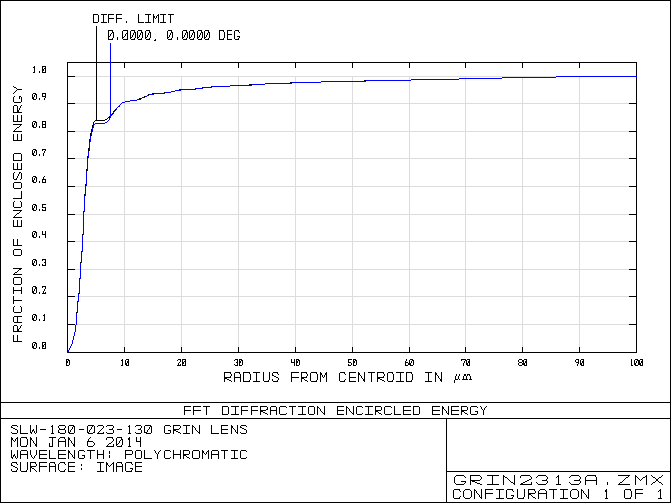
\includegraphics[width=0.75\textwidth]{Images/Zemax/GRO-encircledenergy.png}
\caption{A graph of the energy encircled at a given radius for the actual lens, and for diffraction only. This shows performance that is very nearly diffraction limited.}
\end{figure}

\subsection{Motion resolution}
\label{sec:motion_res}

The motion resolution is dependent on the spectral noise floor of the captured signal.